\section{User Experience}
\label{sec:chapter_2_section_1}

Nello sviluppo dell'interfaccia utente ci si è concentrati nel fornire all'utente una \emph{User Experience} tale
da semplificare il compito di modellazione di un edificio.
L'interfaccia richiede l'utente utilizzi il più possibile l'interfaccia bidimensionale la quale permette
di definire il piano e posizionare gli elementi architettonici complessi (chiamati \emph{building elements}) su di essa.
Tali \emph{building elements} possono essere trovati in un catalogo pre-riempito, ed essere
configurati ulteriormente e personalizzati attraverso il pannello laterale. Questo approccio
di modellazione sposta la complessità verso lo sviluppatore dei \emph{bulding elements} personalizzabili,
lasciando all'utente finale il compito di posizionare e configurare gli elementi utilizzati.
Un ricco catalogo di elementi \`e quindi fondamentale per rispondere alle esigenze di modellazione degli utenti.
Una volta che la scena \`e stata definita in base all'approccio \emph{place-and-configure}, il sistema pu\`o automaticamente
generare un modello 3D che pu\`o essere esplorato esternamente o in prima persona,
(Figura~\ref{fig:3D-school}).\\\\

\begin{figure}[htbp] %  figure placement: here, top, bottom, or page
   \centering
   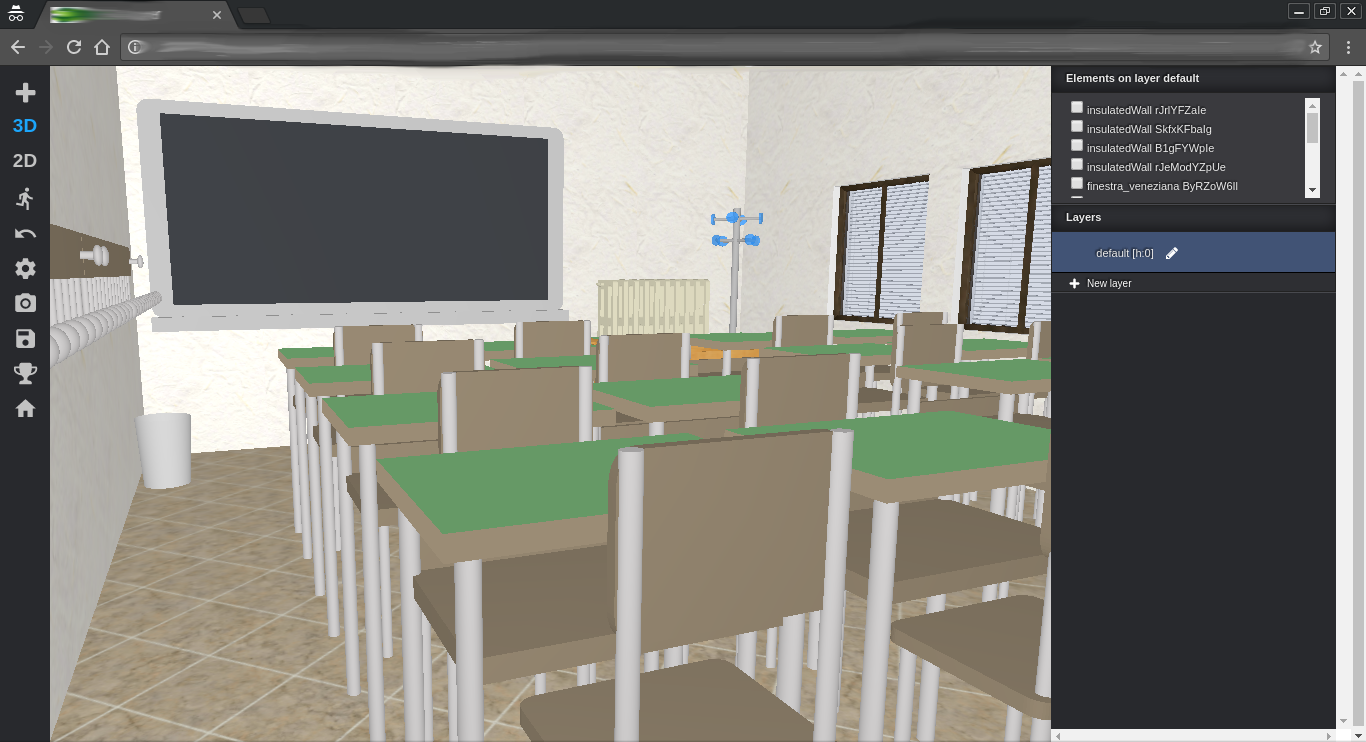
\includegraphics[width=1\linewidth]{images/3d-school}
   \caption{Schermata con visuale in prima persona}
   \label{fig:3D-school}
\end{figure}

Ogni \emph{building element} infatti comprende sia un \emph{funzione generatrice 2D (2Dgf)} e un
\emph{funzione generatrice 3D (3Dgf)}, utilizzate per ottenere modelli nella planimetria 2D e in 3D che ha generato il modello
rispettivamente.
